\documentclass[a4paper,12pt]{article}
\usepackage{amsmath,amssymb,amsfonts,amsthm}
\usepackage{tikz}
\usepackage [utf8x] {inputenc}
\usepackage [T2A] {fontenc} 
\usepackage[russian]{babel}
\usepackage{cmap, upgreek}
\usepackage{textcomp} 

% Так ссылки в PDF будут активны
\usepackage[unicode]{hyperref}

% вы сможете вставлять картинки командой \includegraphics[width=0.7\textwidth]{ИМЯ ФАЙЛА}
% получается подключать, как минимум, файлы .pdf, .jpg, .png.
\usepackage{graphicx}
% Если вы хотите явно указать поля:
\usepackage[margin=1in]{geometry}
% Или если вы хотите задать поля менее явно (чем больше DIV, тем больше места под текст):
% \usepackage[DIV=10]{typearea}

\usepackage{fancyhdr}

\newcommand{\bbR}{\mathbb R}%теперь вместо длинной команды \mathbb R (множество вещественных чисел) можно писать короткую запись \bbR. Вместо \bbR вы можете вписать любую строчку букв, которая начинается с '\'.
\newcommand{\eps}{\varepsilon}
\newcommand{\bbN}{\mathbb N}
\newcommand{\dif}{\mathrm{d}}

\newtheorem{Def}{Определение}


\pagestyle{fancy}
\makeatletter % сделать "@" "буквой", а не "спецсимволом" - можно использовать "служебные" команды, содержащие @ в названии
\fancyhead[L]{\footnotesize Электричество и магнетизм}%Это будет написано вверху страницы слева
\fancyhead[R]{\footnotesize ФМХФ МФТИ}
\fancyfoot[L]{\footnotesize \@author}%имя автора будет написано внизу страницы слева
\fancyfoot[R]{\thepage}%номер страницы —- внизу справа
\fancyfoot[C]{}%по центру внизу страницы пусто

\renewcommand{\maketitle}{%
	\noindent{\bfseries\scshape\large\@title\ \mdseries\upshape}\par
	\noindent {\large\itshape\@author}
	\vskip 2ex}
\makeatother
\def\dd#1#2{\frac{\partial#1}{\partial#2}}


\title{3.4.1 \\ Диа- и парамагнетик}
\author{Егор Берсенев} 
\date{15 апреля 2016 г.}

\begin{document}
	\maketitle
	\section{Цель работы}
	Измерение магнитной восприимчивость диа- и парамагнитного образца.
	\section{Оборудование}
	Электромагнит, аналитические весы, милливеберметр, источник постоянного тока, образцы.
	\section{Теоретическая часть}
	Магнитная восприимчивость может быть определена методом измерения сил, действующих на тело в магнитном поле. Есть два классических метода: метод Фарадея и метод Гюи. Недостаток метода Фарадея состоит в том, что для расчета магнитной восприимчивости необходимо знать величину градиента магнитного поля. Мы же воспользуемся методом Гюи. Он состоит в том, что один из концов тонкого и длинного стержня помещают в зазор электромагнита с постоянным полем, а другой конец вне зазора, где полем можно пренебречь. Найдем выражение для магнитной силы, действующей на такой образец.
	
	Пусть площадь образца равна S, его магнитная восприимчивость $\mu$, а поле в зазоре равно B. При смещении образца вниз на $\Delta l $ вниз магнитная сила, действующая на него, равна $$ F = \left(\frac{\Delta W_m}{\Delta l}\right)_I,$$ где $\Delta W_m$ --- изменение магнитной энергии системы при постоянном токе, и следовательно, при постоянном поле в зазоре.
	Магнитная энергия рассчитывается по формуле: 
	$$
	W_m = \frac{1}{2}\int HB\dif V = \frac{1}{2\mu_0}\int\frac{B^2}{\mu}\dif V
	$$
	Интеграл берется по всему пространству, но при смещении образца магнитная энергия меняется только в области зазора, а около верхнего конца стержня остается неизменным, поскольку поля там нет. Принимая поле внутри стержня равным полю в зазоре, получим:
	$$
	\Delta W_m = \frac{1}{2\mu_0}\frac{B^2}{\mu}s\Delta l - \frac{1}{2\mu_0}B^2s\Delta l = \frac{1-\mu}{2\mu_0\mu}B^2s\Delta l = -\frac{\chi}{2\mu_0\mu}B^2s\Delta l
	$$
	А следовательно, на образец действует сила:
	$$
	F = -\frac{\chi}{2\mu_0\mu}B^2s
	$$
	Пренебрежем тем, что $\mu$ отличается от 1. 
	Схема установки:
	
	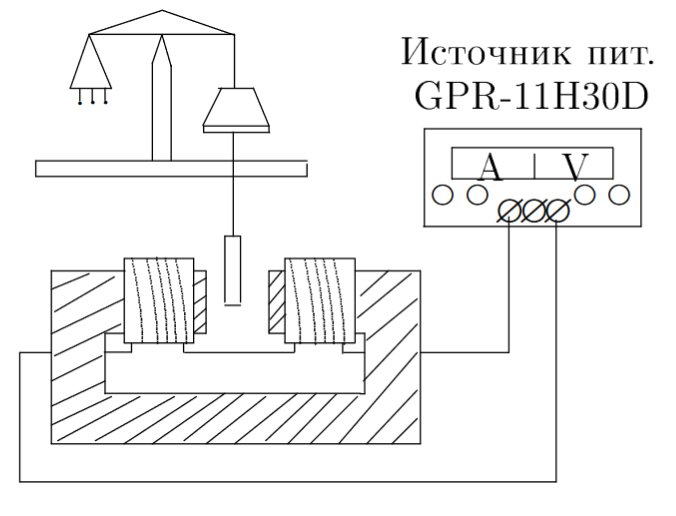
\includegraphics[width = 0.5\linewidth]{pic1}
	
	Измеряя перегрузку $\Delta P = F$ найдем силу, действующую на образец.
	\section{Ход работы}
	Проведем калибровку электромагнита.
		
		\begin{table}[h]
			\centering
			\caption{Калибровка электромагнита}
			\label{my-label}
			\begin{tabular}{|l|l|l|l|l|l|l|l|l|l|l|l|}
				\hline
				$\Phi$, мВб & 0.25 & 0.5  & 0.7  & 0.9  & 1.2  & 1.4  & 1.85 & 2.3  & 2.7  & 3.2  & 3.6  \\ \hline
				I, А     & 0.1  & 0.2  & 0.3  & 0.4  & 0.5  & 0.6  & 0.8  & 1    & 1.2  & 1.4  & 1.6  \\ \hline
				B, Тл     & 0.03 & 0.07 & 0.10 & 0.13 & 0.17 & 0.19 & 0.26 & 0.32 & 0.38 & 0.44 & 0.50 \\ \hline
			\end{tabular}
		\end{table}
		
		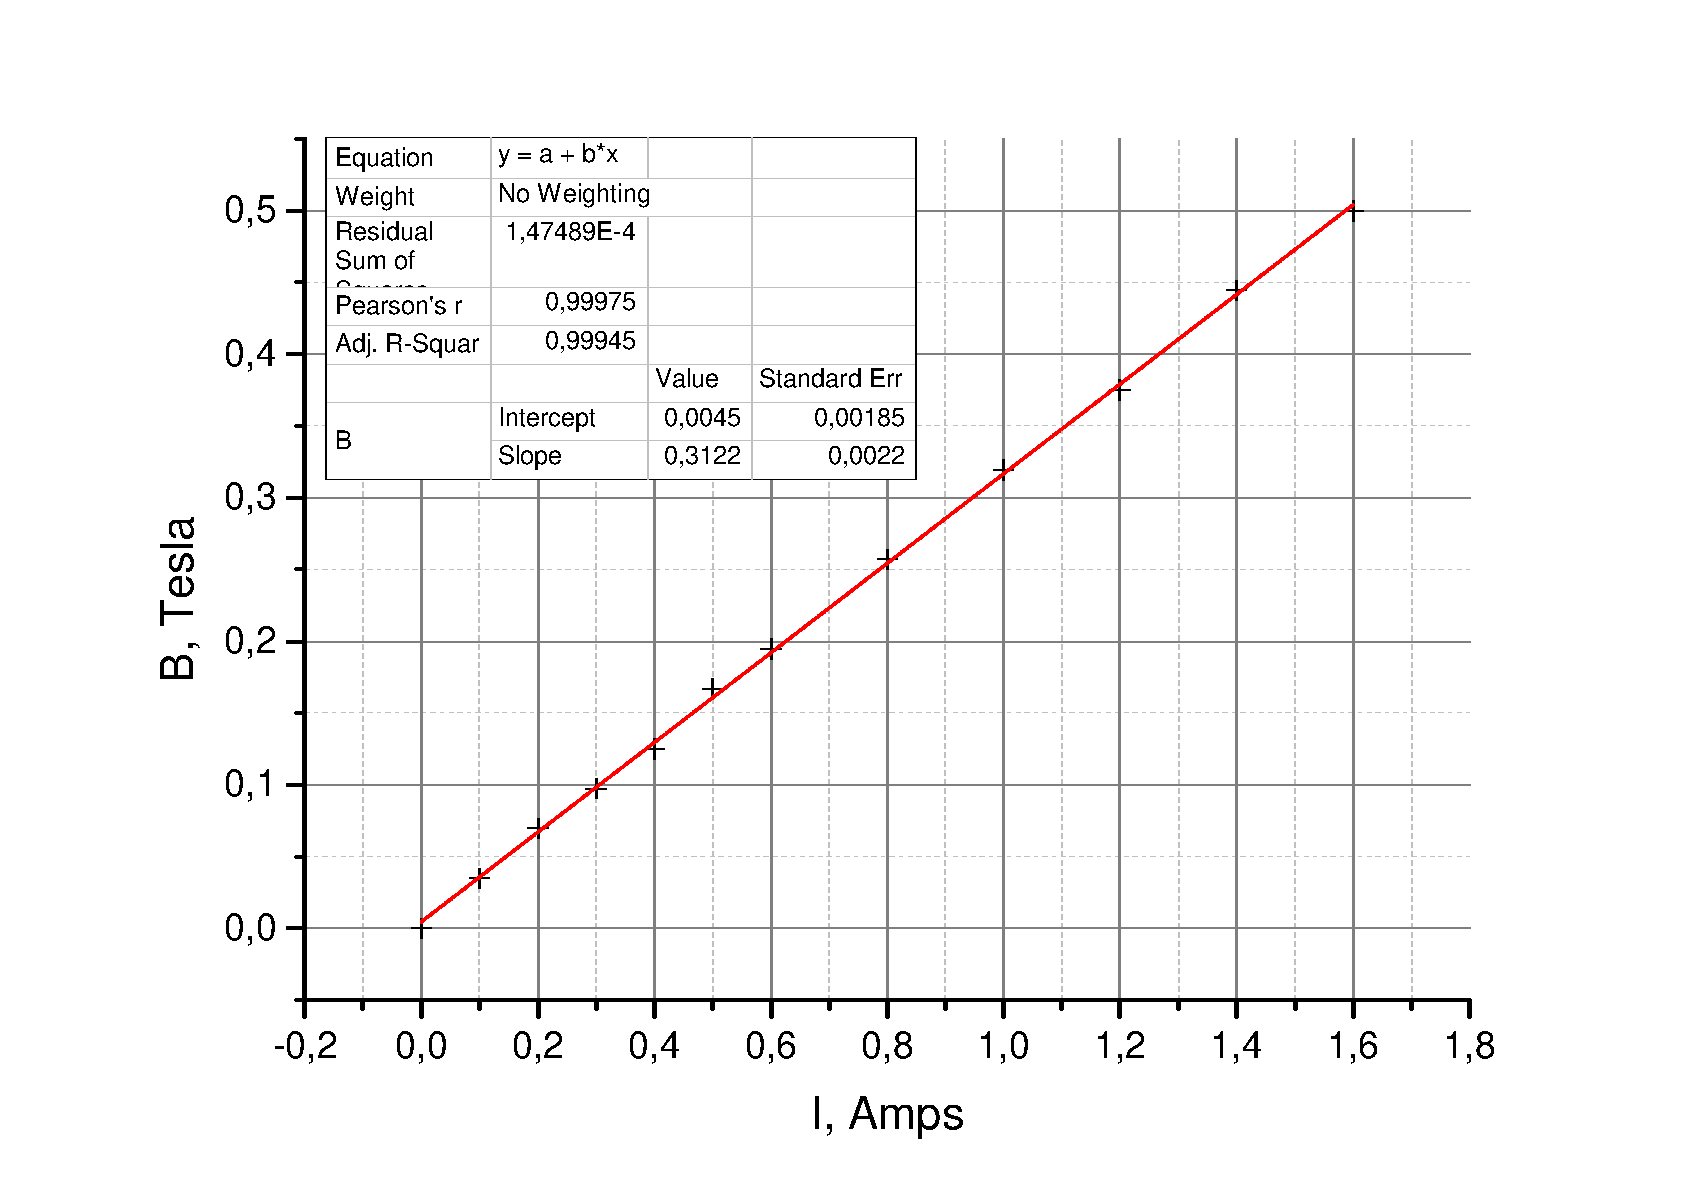
\includegraphics[width = 0.7\linewidth]{graph1}
	
	Диаметр обоих цилиндров равен 1 см.	
		
	Проведем измерения с медным цилиндром:
	
	\begin{table}[h!]
		\centering
		\caption{Медный цилиндр}
		\label{my-label}
		\begin{tabular}{|l|l|l|l|l|l|l|}
			\hline
			$I$   & $m$    & $\Delta m$   & $\Delta P $      & $B$     & $B^2$ & $\Delta P\cdot10^{-5}$ \\ \hline
			0   & -0,5 & 0    & 0        & 0,000 & 0,0000              & 0                       \\ \hline
			0,1 & -0,6 & -0,1 & $-9,8\cdot10^{-7}$ & 0,035 & 0,0012              & -0,10                   \\ \hline
			0,2 & -0,7 & -0,2 & $-2\cdot10^{-6} $  & 0,069 & 0,0048              & -0,20                   \\ \hline
			0,3 & -0,9 & -0,4 & $-3,9\cdot10^{-6}$ & 0,097 & 0,0095              & -0,39                   \\ \hline
			0,4 & -1,1 & -0,6 & $-5,9\cdot10^{-6} $& 0,125 & 0,0156              & -0,59                   \\ \hline
			0,5 & -1,6 & -1,1 & $-1,1\cdot10^{-6} $& 0,167 & 0,0278              & -1,08                   \\ \hline
			0,6 & -1,8 & -1,3 & $-1,3\cdot10^{-6} $& 0,194 & 0,0378              & -1,28                   \\ \hline
			0,8 & -2,3 & -1,8 & $-1,8\cdot10^{-6} $& 0,257 & 0,0660              & -1,77                   \\ \hline
			1   & -3,3 & -2,8 & $-2,7\cdot10^{-6} $& 0,319 & 0,1020              & -2,75                   \\ \hline
			1,2 & -4,6 & -4,1 & $-4\cdot10^{-6} $& 0,375 & 0,1406              & -4,02                   \\ \hline
			1,4 & -6,3 & -5,8 & $-5,7\cdot10^{-6} $& 0,444 & 0,1975              & -5,69                   \\ \hline
		\end{tabular}
	\end{table}
	
	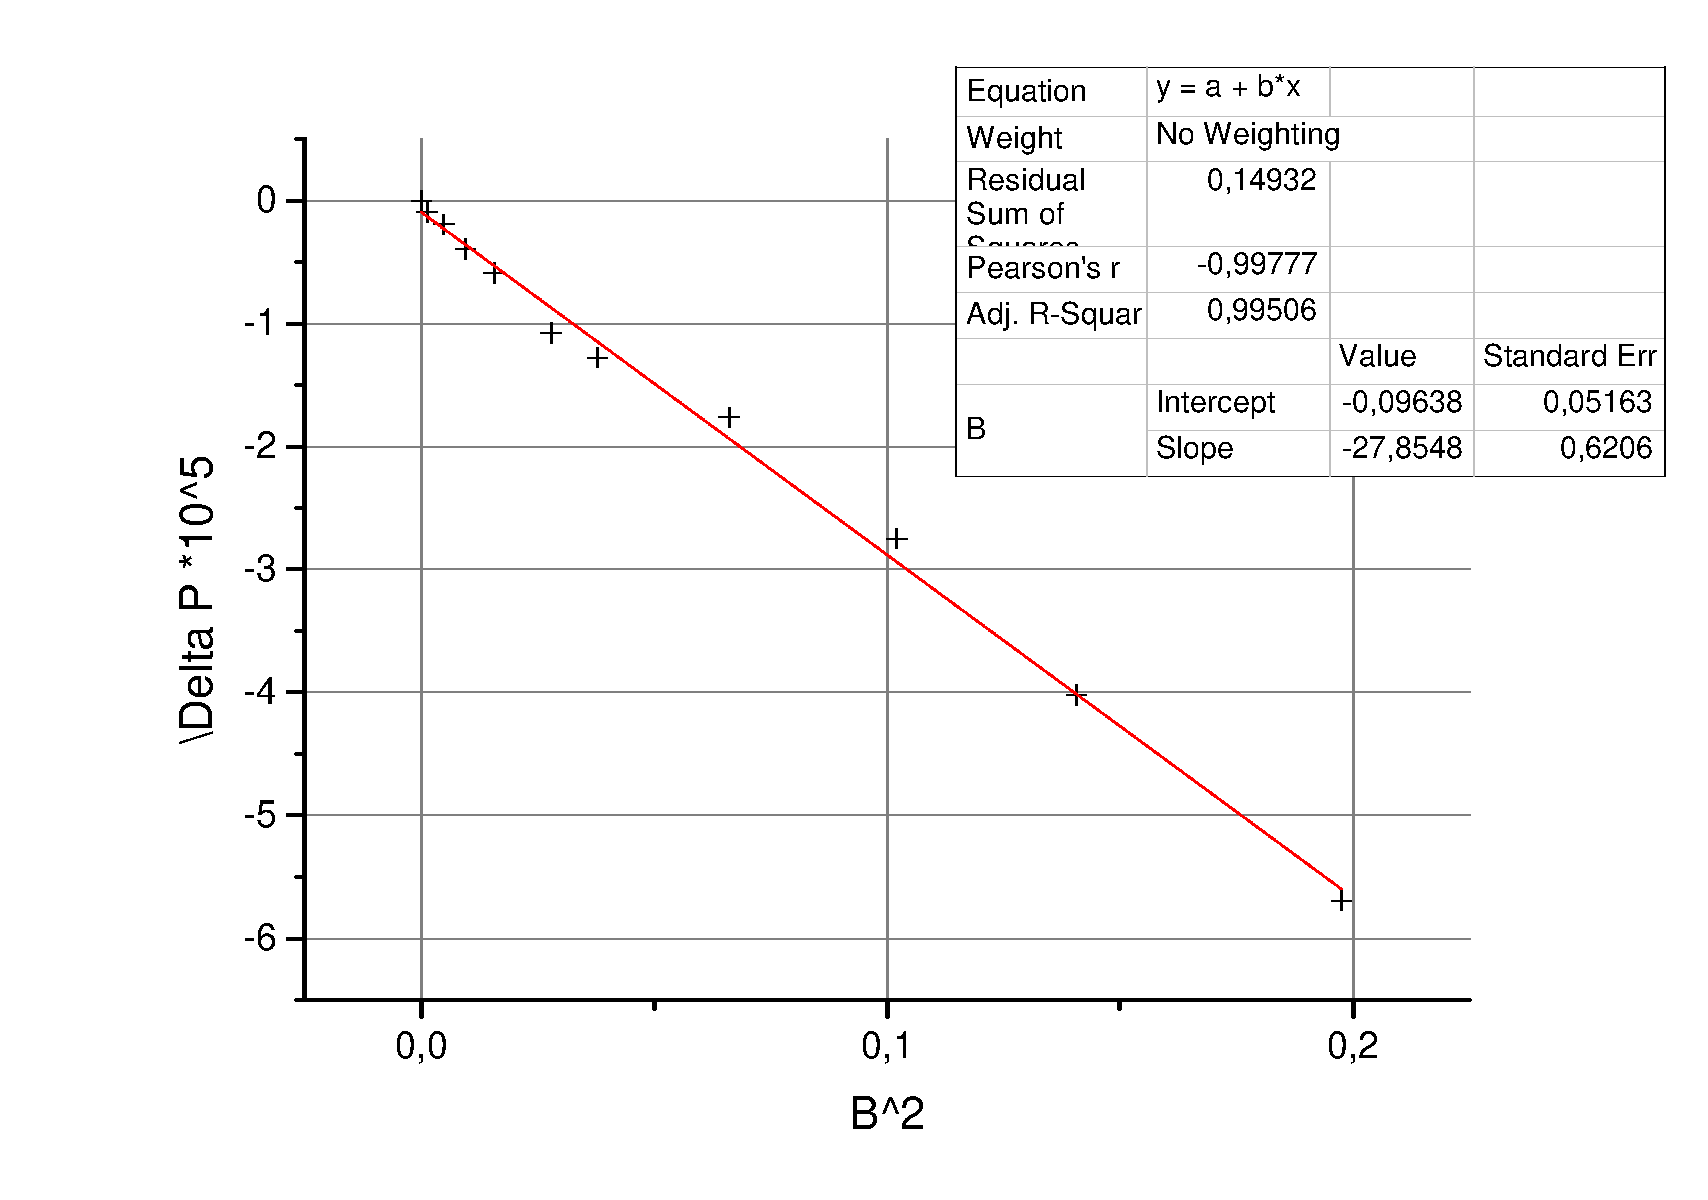
\includegraphics[width = 0.7\linewidth]{graph2}
	
	Рассчитаем магнитную восприимчивость:
	
	$$
	\chi = \frac{8k\cdot 10^{-5}\mu_0}{\pi d^2} = \left(8.914\pm0.922\right)\cdot 10^{-6}
	$$
	\newpage
	Проведем измерения с алюминиевым цилиндром:
	
	\begin{table}[h!]
		\centering
		\caption{My caption}
		\label{my-label}
		\begin{tabular}{|l|l|l|l|l|l|l|}
			\hline
			$I$   & $m$    & $\Delta m$   & $\Delta P $      & $B$     & $B^2$ & $\Delta P\cdot10^{-5}$ \\ \hline
			0   & -0,1 & 0   & 0        & 0,000 & 0,0000              & 0                       \\ \hline
			0,1 & 0,2  & 0,3 & $2,94\cdot 10^{-6}$ & 0,035 & 0,0012              & 0,29                    \\ \hline
			0,2 & 0,3  & 0,4 & $3,92\cdot 10^{-6}$ & 0,069 & 0,0048              & 0,39                    \\ \hline
			0,3 & 1,2  & 1,3 & $1,28\cdot 10^{-5}E-05$ & 0,097 & 0,0095              & 1,28                    \\ \hline
			0,4 & 1,9  & 2   & $1,96\cdot 10^{-5}$ & 0,125 & 0,0156              & 1,96                    \\ \hline
			0,5 & 2,4  & 2,5 & $2,45\cdot 10^{-5}$ & 0,167 & 0,0278              & 2,45                    \\ \hline
			0,6 & 3,1  & 3,2 & $3,14\cdot 10^{-5}$ & 0,194 & 0,0378              & 3,14                    \\ \hline
			0,8 & 5,5  & 5,6 & $5,49\cdot 10^{-5}$ & 0,257 & 0,0660              & 5,49                    \\ \hline
			1   & 8,1  & 8,2 & $8,04\cdot 10^{-5}$ & 0,319 & 0,1020              & 8,04                    \\ \hline
		\end{tabular}
\end{table}	
		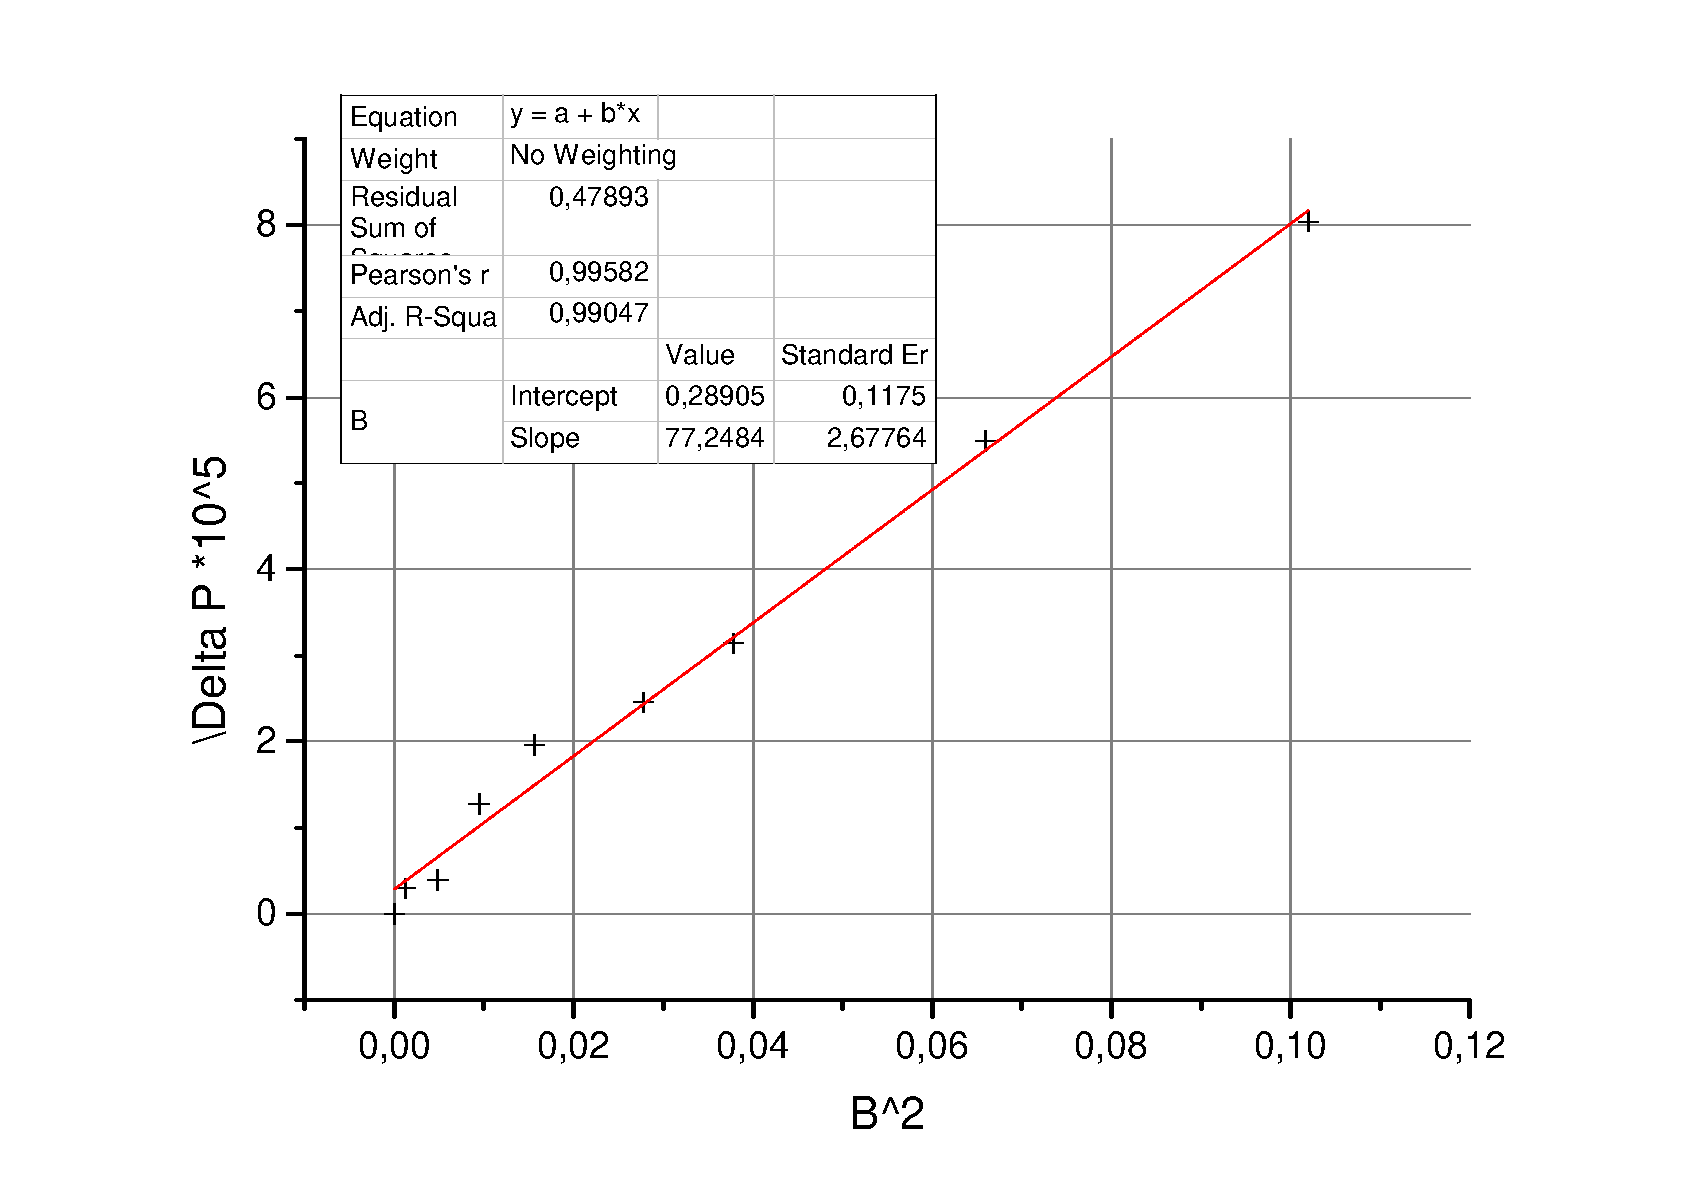
\includegraphics[width = 0.7\linewidth]{graph3}
		
		Рассчитаем магнитную восприимчивость:
		
		$$
		\chi = \frac{8k\cdot 10^{-5}\mu_0}{\pi d^2} = \left(2.472\pm0.360\right)\cdot 10^{-5}
		$$

	
	\section{Вывод}
	Метод Гюи дает возможность получать достоверные значения магнитной восприимчивости. Табличные значения: $\chi_{Cu} = -9.2\cdot10^{-6}$, $\chi_{Al} = 2.22\cdot 10^{-5}$. Полученные результаты сходятся с ними в пределах погрешности.
\end{document}